\documentclass[a4paper, 14pt]{extarticle}

% Поля
%--------------------------------------
\usepackage{geometry}
\geometry{a4paper,tmargin=2cm,bmargin=2cm,lmargin=3cm,rmargin=1cm}
%--------------------------------------


%Russian-specific packages
%--------------------------------------
\usepackage[T2A]{fontenc}
\usepackage[utf8]{inputenc} 
\usepackage[english, main=russian]{babel}
%--------------------------------------

\usepackage{textcomp}

% Красная строка
%--------------------------------------
\usepackage{indentfirst}               
%--------------------------------------             


%Graphics
%--------------------------------------
\usepackage{graphicx}
\graphicspath{ {./images/} }
\usepackage{wrapfig}
%--------------------------------------

% Полуторный интервал
%--------------------------------------
\linespread{1.3}                    
%--------------------------------------

%Выравнивание и переносы
%--------------------------------------
% Избавляемся от переполнений
\sloppy
% Запрещаем разрыв страницы после первой строки абзаца
\clubpenalty=10000
% Запрещаем разрыв страницы после последней строки абзаца
\widowpenalty=10000
%--------------------------------------

%Списки
\usepackage{enumitem}

%Подписи
\usepackage{caption} 

%Гиперссылки
\usepackage{hyperref}

\hypersetup {
	unicode=true
}

%Рисунки
%--------------------------------------
\DeclareCaptionLabelSeparator*{emdash}{~--- }
\captionsetup[figure]{labelsep=emdash,font=onehalfspacing,position=bottom}
%--------------------------------------

\usepackage{tempora}
\usepackage{amsmath}
\usepackage{color}
\usepackage{listings}
\lstset{
  belowcaptionskip=1\baselineskip,
  breaklines=true,
  frame=L,
  xleftmargin=\parindent,
  language=Python,
  showstringspaces=false,
  basicstyle=\footnotesize\ttfamily,
  keywordstyle=\bfseries\color{blue},
  commentstyle=\itshape\color{purple},
  identifierstyle=\color{black},
  stringstyle=\color{red},
}

%--------------------------------------
%			НАЧАЛО ДОКУМЕНТА
%--------------------------------------

\begin{document}

%--------------------------------------
%			ТИТУЛЬНЫЙ ЛИСТ
%--------------------------------------
\begin{titlepage}
\thispagestyle{empty}
\newpage


%Шапка титульного листа
%--------------------------------------
\vspace*{-60pt}
\hspace{-65pt}
\begin{minipage}{0.3\textwidth}
\hspace*{-20pt}\centering

\includegraphics[width=\textwidth]{emblem}
\end{minipage}
\begin{minipage}{0.67\textwidth}\small \textbf{
\vspace*{-0.7ex}
\hspace*{-6pt}\centerline{Министерство науки и высшего образования Российской Федерации}
\vspace*{-0.7ex}
\centerline{Федеральное государственное бюджетное образовательное учреждение }
\vspace*{-0.7ex}
\centerline{высшего образования}
\vspace*{-0.7ex}
\centerline{<<Московский государственный технический университет}
\vspace*{-0.7ex}
\centerline{имени Н.Э. Баумана}
\vspace*{-0.7ex}
\centerline{(национальный исследовательский университет)>>}
\vspace*{-0.7ex}
\centerline{(МГТУ им. Н.Э. Баумана)}}
\end{minipage}
%--------------------------------------

%Полосы
%--------------------------------------
\vspace{-25pt}
\hspace{-35pt}\rule{\textwidth}{2.3pt}

\vspace*{-20.3pt}
\hspace{-35pt}\rule{\textwidth}{0.4pt}
%--------------------------------------

\vspace{1.5ex}
\hspace{-35pt} \noindent \small ФАКУЛЬТЕТ\hspace{80pt} <<Информатика и системы управления>>

\vspace*{-16pt}
\hspace{47pt}\rule{0.83\textwidth}{0.4pt}

\vspace{0.5ex}
\hspace{-35pt} \noindent \small КАФЕДРА\hspace{50pt} <<Теоретическая информатика и компьютерные технологии>>

\vspace*{-16pt}
\hspace{30pt}\rule{0.866\textwidth}{0.4pt}
  
\vspace{11em}

\begin{center}
\Large {\bf Лабораторная работа № 3} \\ 
\large {\bf по курсу <<Языки и методы программирования>>} \\ 
\large <<Полиморфизм на основе интерфейсов в языке Java>>
\end{center}\normalsize

\vspace{8em}


\begin{flushright}
  {Студент группы ИУ9-21Б Хромов М.А.\hspace*{15pt} \\
  \vspace{2ex}
  Преподаватель Посевин Д. П.\hspace*{15pt}}
\end{flushright}

\bigskip

\vfill
 

\begin{center}
\textsl{Москва 2025}
\end{center}
\end{titlepage}
%--------------------------------------
%		КОНЕЦ ТИТУЛЬНОГО ЛИСТА
%--------------------------------------

\renewcommand{\ttdefault}{pcr}

\setlength{\tabcolsep}{3pt}
\newpage
\section{Цель}\label{Sect::task}
\par
Приобретение навыков реализации интерфейсов для обеспечения возможности
полиморфной обработки объектов класса.  

\section{Задание}\label{Sect::task}
\par
Во время выполнения лабораторной работы требуется разработать на языке Java один из
классов, перечисленных в таблице. В классе должен быть реализован интерфейс Comparable<T>
и переопределён метод toString. В методе main вспомогательного класса Test нужно
продемонстрировать работоспособность разработанного класса путём сортировки массива его
экземпляров.
\par

\section{Индивидуальный вариант}
\par
Вариант 21
\par 
Класс, представляющий абитуриента, с порядком на основе суммы баллов
по трём ЕГЭ: информатика, математика и русский язык. 
\par
(Нужно
учитывать, что ЕГЭ различаются по приоритетам, позволяющим
упорядочивать абитуриентов, имеющих одинаковые суммы баллов.)


\section {Практическая реализация}
Исходный код программы представлен в листингах~\ref{lst:code1}--~\ref{lst:code2}.
\begin{figure}[!htb]
\begin{lstlisting}[language={},caption={Основной класс для варинта 21 (IntSet)},label={lst:code1}]
import java.util.Arrays;

class Applicant implements Comparable<Applicant> {
    private String name;
    private int informaticsScore;
    private int mathScore;
    private int russianScore;

    public Applicant(String name, int informaticsScore, int mathScore, int russianScore) {
        this.name = name;
        this.informaticsScore = informaticsScore;
        this.mathScore = mathScore;
        this.russianScore = russianScore;

    }

    public int getTotalScore() {
        return informaticsScore + mathScore + russianScore;
    }
    public int compareTo(Applicant other) {
        if (this.getTotalScore() != other.getTotalScore()) {
            return Integer.compare(other.getTotalScore(), this.getTotalScore());
        }
        if (this.informaticsScore != other.informaticsScore) {
            return Integer.compare(other.informaticsScore, this.informaticsScore);
        }
        if (this.mathScore != other.mathScore) {
            return Integer.compare(other.mathScore, this.mathScore);
        }
        return Integer.compare(other.getTotalScore(), this.getTotalScore());
    }
    public String toString() {
        return String.format("{Имя: %s, Инфа: %d, Математика: %d, Русский: %d, Сумма: %d}",
                name, informaticsScore, mathScore, russianScore, getTotalScore());
    }
}


\end{lstlisting}
\end{figure}

\newpage
\begin{figure}[!htb]
\begin{lstlisting}[language={},caption={Тестовый класс для варинта 21 (с консольным интерфейсом},label={lst:code2}]
import java.util.Arrays;
import java.util.Scanner;

public class Test {
    public static void main(String[] args) {
        Scanner scanner = new Scanner(System.in);

        System.out.print("Введите количество абитуриентов: ");
        int count = scanner.nextInt();
        scanner.nextLine();

        Applicant[] applicants = new Applicant[count];

        for (int i = 0; i < count; i++) {
            System.out.println("Введите данные абитуриента " + (i + 1) + ":");

            System.out.print("Имя: ");
            String name = scanner.nextLine();

            System.out.print("Баллы по информатике: ");
            int inf = scanner.nextInt();

            System.out.print("Баллы по математике: ");
            int math = scanner.nextInt();

            System.out.print("Баллы по русскому языку: ");
            int rus = scanner.nextInt();
            scanner.nextLine();

            applicants[i] = new Applicant(name, inf, math, rus);
        }
        Arrays.sort(applicants);
        System.out.println("\nСписок абитуриентов:");
        for (Applicant a : applicants) {
            System.out.println(a);
        }

        scanner.close();
    }
}



\end{lstlisting}
\end{figure}

\clearpage
\newpage

\section{Реализация  интерактивной консолью}
\begin{center}
    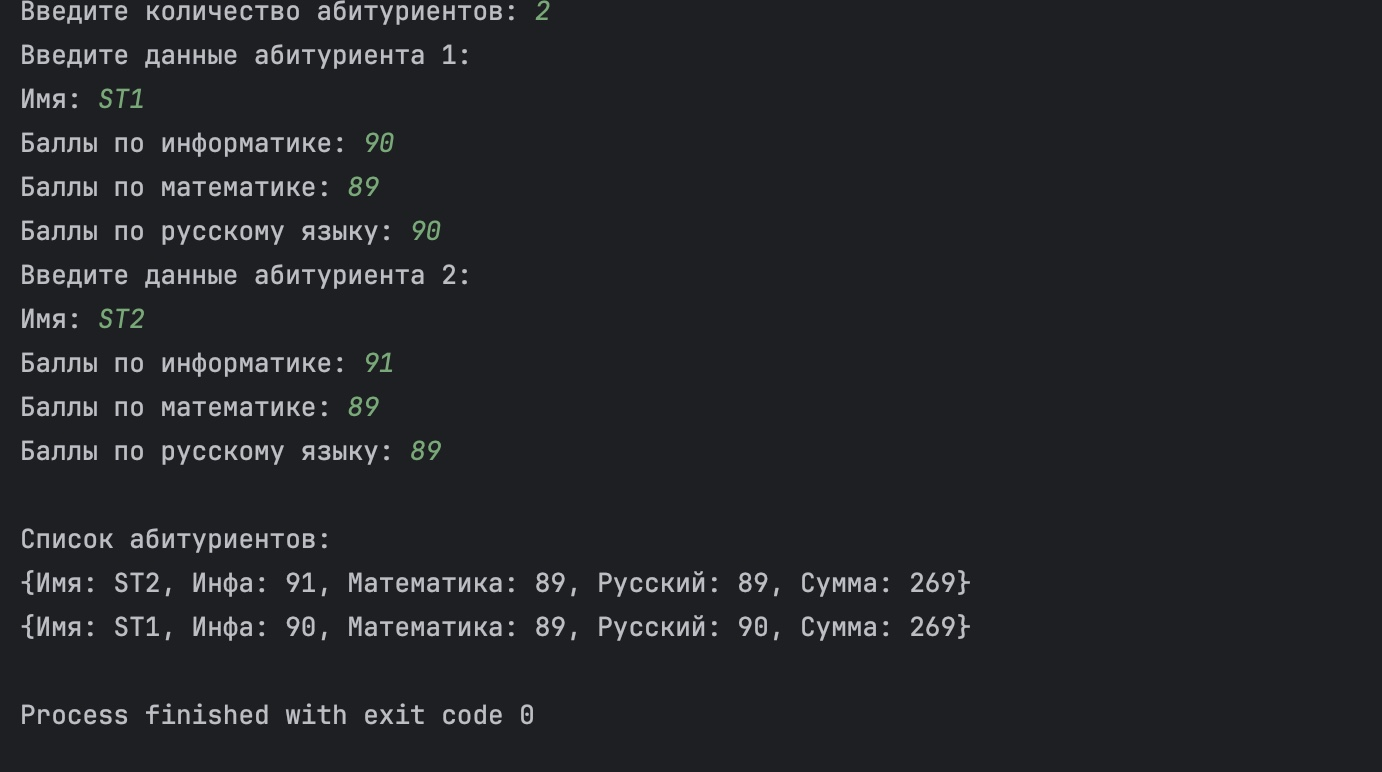
\includegraphics[width=0.8\textwidth]{фото5.jpeg}
    \captionof{figure}{Запуск программы}
\end{center}
\newpage
\section{Вывод}
В данной работе реализован класс Abiturient, представляющий абитуриента. Класс имплементирует интерфейс Comparable<Abiturient>, что позволяет сортировать объекты по сумме баллов ЕГЭ (информатика, математика, русский язык). В случае одинаковых сумм используется приоритетность предметов.
\parla
В классе Test реализован консольный интерфейс, позволяющий вводить данные об абитуриентах, выводить список до и после сортировки, а также демонстрирующий корректность работы переопределённых методов.
\end{document}